\chapter{Testing}
\label{testing}
%TODO: redo all tests and include final tikz as test result
\section{Setup}
The original paper discussing STP is openly available.
However, it does not dictate exact implementation details.
Therefore, in order to reach an accurate enough understanding of it multiple tests were performed.
To minimize external influences these tests needed to be done in a network disconnected from any external network.
Additionally, to be able to check the results for correctness, we kept the network small and simple.
The layout of the test setup can be seen in Figure~\ref{fig:test_setup}.
While a very basic network, it is sufficient for the tests described below, which will guarantee the required capabilities of the developed tool.
The root in figure~\ref{fig:test_setup} was made root by manually assigning it a higher priority than the other bridges (note that \textit{higher} in this case means \textit{smaller}).
Bridges \textit{A}, \textit{B} and \textit{C} had their priorities left to the default value.
Nodes \textit{A}, \textit{B} and \textit{C} were running \textit{Wireshark} and the developed tool.
Additionally using \textit{Wireshark} allowed us to check the actual packages involved in the testing process to monitor progress and note situations not handled correctly by the tool.
The server for our tool was run on Node \textit{A}.
Test results were checked for their correctness by checking the report provided by the tool.

\begin{figure}[h]
    \centering
    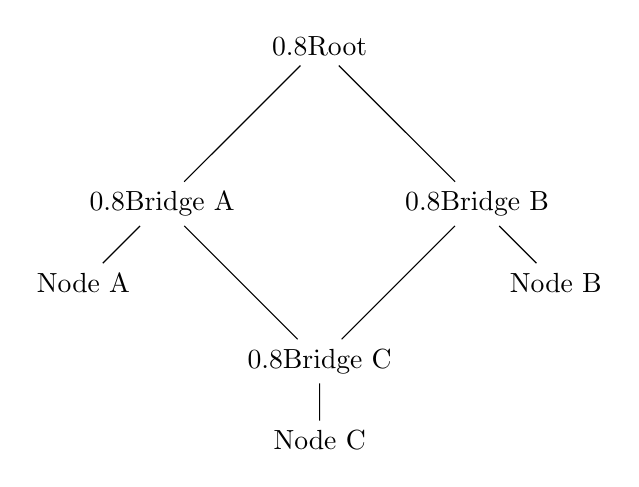
\begin{tikzpicture}
        \node (root) at (2, 4) {\switch{0.8}{Root}};
        \node (a) at (0, 2) {\switch{0.8}{Bridge A}};
        \node (na) at (-1, 1) {Node A};
        \node (b) at (4, 2) {\switch{0.8}{Bridge B}};
        \node (nb) at (5, 1) {Node B};
        \node (c) at (2, 0) {\switch{0.8}{Bridge C}};
        \node (nc) at (2, -1) {Node C};
    \draw 
    (root) -- (a)
    (root) -- (b)
    (a) -- (c)
    (b) -- (c)
    (a) -- (na)
    (b) -- (nb)
    (c) -- (nc);
    \end{tikzpicture}
    \caption{Test setup}
    \label{fig:test_setup}
\end{figure}

\section{Tests}
\subsection*{"Plug and Play" Test}
\label{usage_test}
This test is meant to ensure the general bridge discovery ability of our tool.
It is designed to simulate the connection of nodes to an established network.
Using a simple setup like shown in Figure~\ref{fig:test_setup} allows us to collect information about the whole network.
If we were using less nodes than we had non-root bridges in the network, this would not be possible.

\subsubsection*{Performing the test}
\begin{enumerate}
    \item The layout shown in Figure~\ref{fig:test_setup} was established and all devices were started.
    \item No tool was started yet, identification during the tree establishment is covered by the Tree Establishment Test (\ref{tree_est_test})
    \item We waited for the bridges to establish a stable spanning tree, checking the progress by observing the STP packets for the TC flag.
    \item After the tree had stabilized we started the server on node \textit{A} and the tools on all the nodes.
    \item We waited for the tools to send their data to the server, which takes one $helloTime$ plus the latency between the nodes and the server. Default value for the $helloTime$ is 2 seconds.
    \item When all nodes had sent their data to the server we created a report to check it against the expected result.
\end{enumerate}
\subsubsection*{Expected Result}
With the limited size of the test network all bridges can and must be identified correctly for this test to be counted as successful.
If the bridges in the network behave as they should, the tool should not be able to gather information about connections between the bridges.

\subsubsection*{Actual Result}
All nodes are correctly identified.
As the tree is already established when the tools are started, no information about connections between the bridges can be gathered.
See Figure~\ref{fig:pnp}.
\begin{figure}[h]
    \centering
    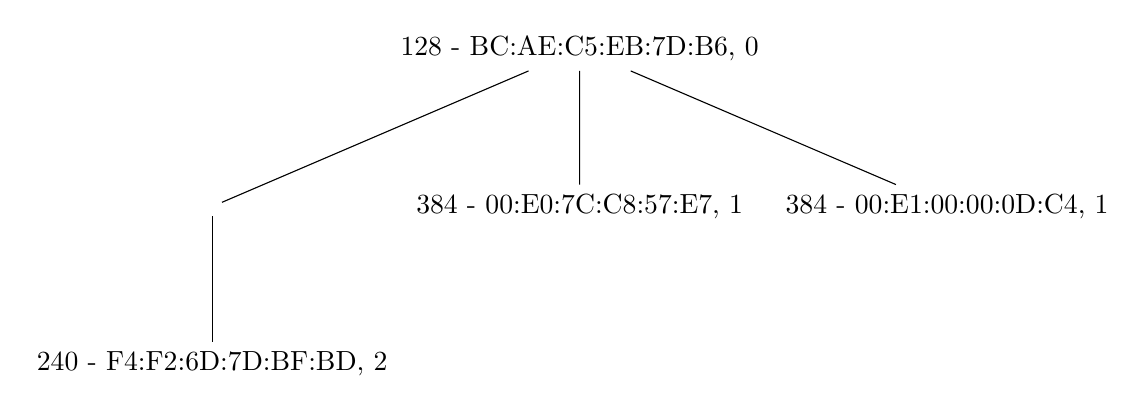
\begin{tikzpicture}
        \node (0) at (7.000000,20) {128 - BC:AE:C5:EB:7D:B6, 0};
        \node (1) at (2.333333,18) {};
        \node (2) at (2.333333,16) {240 - F4:F2:6D:7D:BF:BD, 2};
        \draw (1) -- (2);
        \node (3) at (7.000000,18) {384 - 00:E0:7C:C8:57:E7, 1};
        \node (4) at (11.666667,18) {384 - 00:E1:00:00:0D:C4, 1};
        \draw 
        (0) -- (1)
        (0) -- (3)
        (0) -- (4);
    \end{tikzpicture}
    \caption{The visualization after completing the "Plug and Play" test}
    \label{fig:pnp}
\end{figure}

\subsection*{Tree Establishment Test}
\label{tree_est_test}
To test whether the tool can handle bridges being added to the network during runtime, we start the tool on all nodes before the establishment of the spanning tree, and check for correct identification afterwards.

\subsubsection*{Performing the test}
\begin{enumerate}
    \item The layout shown in Figure~\ref{fig:test_setup} was established and all devices were started.
    \item Before enabling STP on all the bridges we started the server and tools.
    \item After enabling STP on the bridges we waited for the tree to be established, again checking the progress via the TC flag.
    \item Finally we checked the result for correctness.
\end{enumerate}

\subsubsection*{Expected Result}
Again all the bridges can and must be correctly identified.
Additionally, this time the identification of bridge connections is possible, and the topology should therefore be fully identified.

\subsubsection*{Actual Result}
If bridge \textit{D} is connected to bridges \textit{B} and \textit{C} before they are connected to bridge \textit{A}, the tree can build up slowly and the clients will know about the connections.
The resulting visualization can be seen in Figure~\ref{fig:est}
\begin{figure}[h]
    \centering
    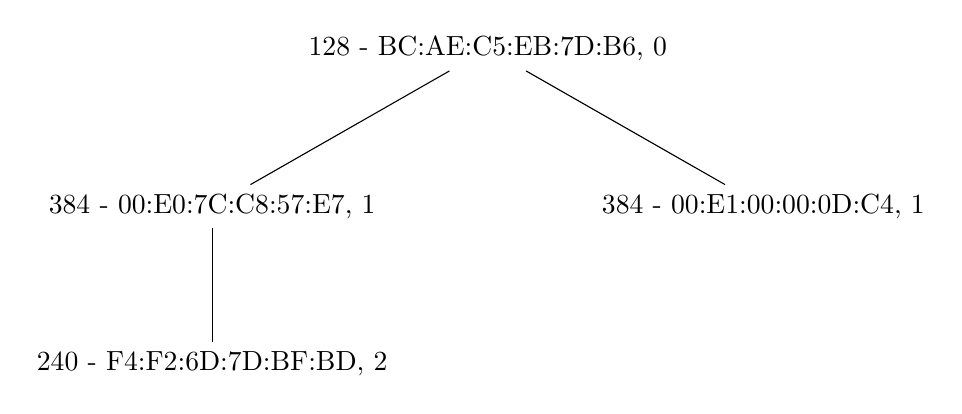
\begin{tikzpicture}[]
        \node (0) at (7.000000,20) {128 - BC:AE:C5:EB:7D:B6, 0};
        \node (1) at (3.500000,18) {384 - 00:E0:7C:C8:57:E7, 1};
        \node (2) at (3.500000,16) {240 - F4:F2:6D:7D:BF:BD, 2};
        \draw 
        (1) -- (2);
        \node (3) at (10.500000,18) {384 - 00:E1:00:00:0D:C4, 1};
        \draw 
        (0) -- (1)
        (0) -- (3);
    \end{tikzpicture}
    \caption{The test setup with fully recognized connections}
    \label{fig:est}
\end{figure}

\subsection*{Bridge Removal Test}
\label{removal_test}
The tool must also be able to handle bridges dropping from a network.
This test makes sure that capability is given.

\subsubsection*{Performing the test}
\begin{enumerate}
    \item We started all the nodes and tools and waited for the spanning tree to be established and correctly identified (see the sections on the Usage Test \ref{usage_test} and the Tree Establishment Test \ref{tree_est_test}).
    \item After the tree was constructed we unplugged Node \textit{B} and waited for the tree to stabilize.
    \item Finally we checked the output of the report for correct identification of the smaller tree.
\end{enumerate}

\subsubsection*{Expected Result}
Bridge \textit{B} must correctly be removed from the topology visualization.

\subsubsection*{Actual Result}
As visible in Figure~\ref{fig:removal}, the bridge is correctly removed.
\begin{figure}[h]
    \centering
    \begin{tikzpicture}[]
        \node (0) at (7.000000,20) {128 - BC:AE:C5:EB:7D:B6, 0};
        \node (1) at (3.500000,18) {};
        \node (2) at (3.500000,16) {240 - F4:F2:6D:7D:BF:BD, 2};
        \draw (1) -- (2);
        \node (3) at (10.500000,18) {384 - 00:E0:7C:C8:57:E7, 1};
        \draw 
        (0) -- (1)
        (0) -- (3);
    \end{tikzpicture}
    \caption{The visualization after bridge \textit{B} is removed}
    \label{fig:removal}
\end{figure}

\subsection*{Slow Dynamic Change Test}
\label{slow_dynamic_test}
Changes in the network topology must not be a problem for the tool.
By successfully testing for additions and removals from the network (sections \ref{usage_test} and \ref{removal_test}) one could assume that changes can be handled as well, but caution demands that we test specifically for changes in the topology.
Node \textit{C} is connected to the root either via node \textit{A} or node \textit{B}.
The node with the smaller MAC address (as they have the same priority) will be the preferred hop to the root.
Therefore the logical topology will look like either one of the figures in Figure~\ref{fig:possible_topologies}.
In our case bridge \textit{C} was logically connected to bridge \textit{A} as that was the possible connection to the root with the smaller MAC address.

\begin{figure}[hp]
    \begin{center}
        \begin{subfigure}[b]{0.4\textwidth}
            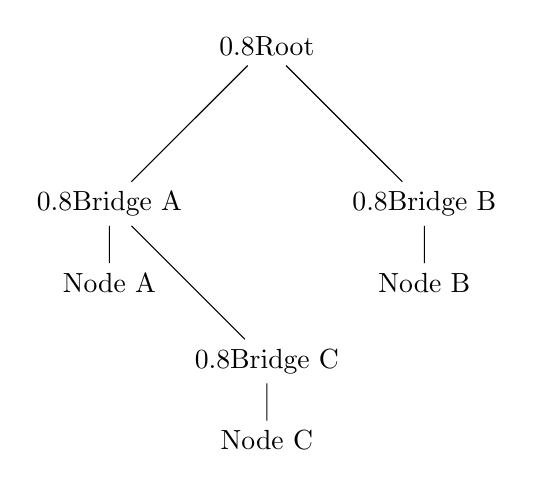
\begin{tikzpicture}
                \node (root) at (2, 4) {\switch{0.8}{Root}};
                \node (a) at (0, 2) {\switch{0.8}{Bridge A}};
                \node (na) at (0, 1) {Node A};
                \node (b) at (4, 2) {\switch{0.8}{Bridge B}};
                \node (nb) at (4, 1) {Node B};
                \node (c) at (2, 0) {\switch{0.8}{Bridge C}};
                \node (nc) at (2, -1) {Node C};
                \draw 
                (root) -- (a)
                (root) -- (b)
                (a) -- (c)
                (a) -- (na)
                (b) -- (nb)
                (c) -- (nc);
            \end{tikzpicture}
            \caption{Path via Bridge A}
        \end{subfigure}
        \hspace{1cm}
        \begin{subfigure}[b]{0.4\textwidth}
            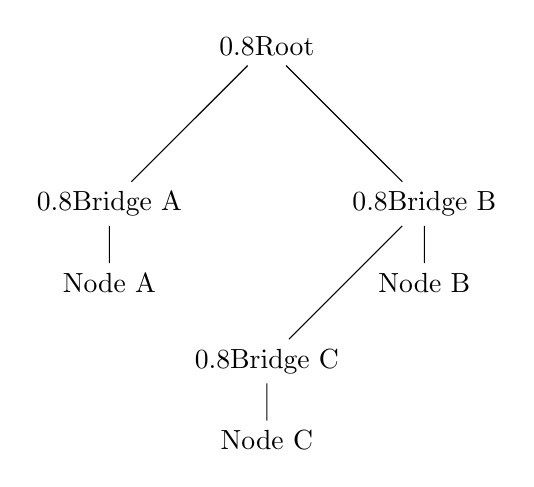
\begin{tikzpicture}
                \node (root) at (2, 4) {\switch{0.8}{Root}};
                \node (a) at (0, 2) {\switch{0.8}{Bridge A}};
                \node (na) at (0, 1) {Node A};
                \node (b) at (4, 2) {\switch{0.8}{Bridge B}};
                \node (nb) at (4, 1) {Node B};
                \node (c) at (2, 0) {\switch{0.8}{Bridge C}};
                \node (nc) at (2, -1) {Node C};
                \draw 
                (root) -- (a)
                (root) -- (b)
                (b) -- (c)
                (a) -- (na)
                (b) -- (nb)
                (c) -- (nc);
            \end{tikzpicture}
            \caption{Path via Bridge B}
       \end{subfigure}
    \end{center}
    \caption{The 2 possible paths to the root from node \textit{C}}
    \label{fig:possible_topologies}
\end{figure}

\subsubsection*{Performing the test}
\begin{enumerate}
    \item We set up all the nodes and waited for a stable tree to be generated by the bridges like before (sections \ref{usage_test}, \ref{tree_est_test} and \ref{removal_test}).
    \item We disconnected bridge \textit{A} from the root, leaving us with a 2 bridge subtree.
    \item The connection between bridges \textit{B} and \textit{C} was also severed, leaving bridges \textit{A} and \textit{C} in a disconnected subtree.
    \item We waited for the spanning tree to stabilize after the removal.
    \item Bridges \textit{A} and \textit{C} were connected to bridge \textit{B} yielding the physical topology shown in Figure~\ref{fig:deep_topology}.
    \item After the tree had stabilized we checked the report output for correctness.
\end{enumerate}

\begin{figure}[hp]
    \begin{center}
        \begin{subfigure}[b]{0.4\textwidth}
            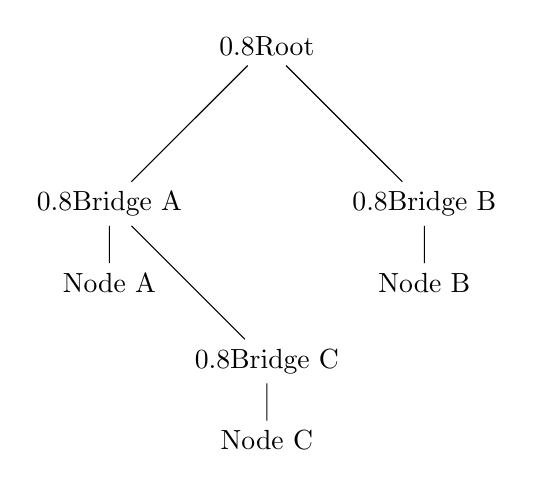
\begin{tikzpicture}
                \node (root) at (2, 4) {\switch{0.8}{Root}};
                \node (a) at (0, 2) {\switch{0.8}{Bridge A}};
                \node (na) at (0, 1) {Node A};
                \node (b) at (4, 2) {\switch{0.8}{Bridge B}};
                \node (nb) at (4, 1) {Node B};
                \node (c) at (2, 0) {\switch{0.8}{Bridge C}};
                \node (nc) at (2, -1) {Node C};
                \draw 
                (root) -- (a)
                (root) -- (b)
                (a) -- (c)
                (a) -- (na)
                (b) -- (nb)
                (c) -- (nc);
            \end{tikzpicture}
            \caption{The topology before the test}
        \end{subfigure}
        \hspace{1cm}
        \begin{subfigure}[b]{0.4\textwidth}
            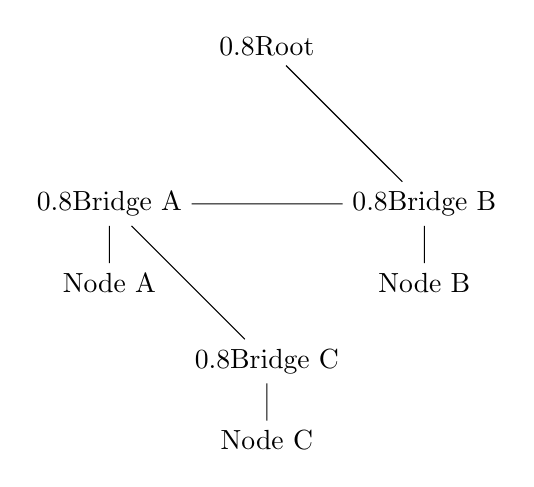
\begin{tikzpicture}
                \node (root) at (2, 4) {\switch{0.8}{Root}};
                \node (a) at (0, 2) {\switch{0.8}{Bridge A}};
                \node (na) at (0, 1) {Node A};
                \node (b) at (4, 2) {\switch{0.8}{Bridge B}};
                \node (nb) at (4, 1) {Node B};
                \node (c) at (2, 0) {\switch{0.8}{Bridge C}};
                \node (nc) at (2, -1) {Node C};

                \draw 
                (root) -- (b)
                (b) -- (a)
                (a) -- (c)
                (a) -- (na)
                (b) -- (nb)
                (c) -- (nc);
            \end{tikzpicture}
            \caption{The topology after the test}
       \end{subfigure}
    \end{center}
    \caption{The topology before and after performing the Slow Dynamic Change Test}
    \label{fig:deep_topology}
\end{figure}

\subsubsection*{Expected Result}
Because we wait for the small subtree to stabilize, establishing bridge \textit{A} as root, the subtree should be correctly identified.

\subsubsection*{Actual Result}
The visualization acquired before executing the test is the same as in Figure~\ref{fig:est}, as we used that test as preparation.
For an unknown reason, the message ages for the subtree that we disconnect \textit{00:E0:7C:C8:57:E7} and \textit{F4:F2:6D:7D:BF:BD} does not get updated and increased.
This needs to be fixed in a future revision of the tool.
The obtained visualization can be seen in Figure~\ref{fig:dynAfter}.
\begin{figure}[h]
    \centering
    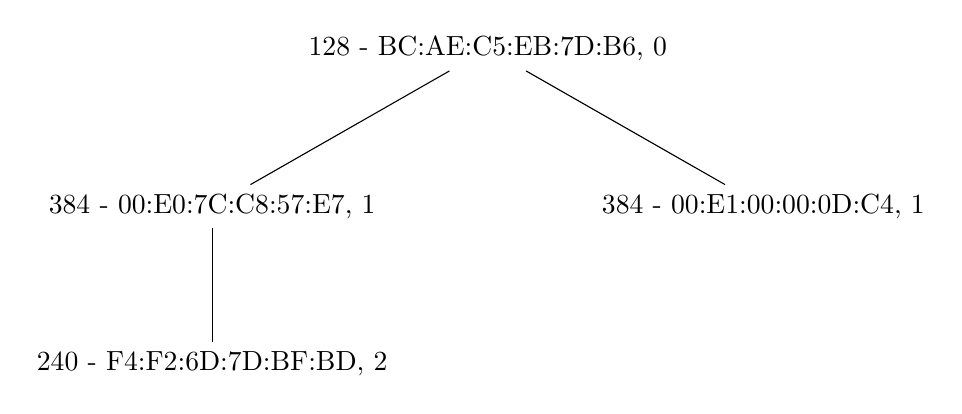
\begin{tikzpicture}[]
        \node (0) at (7.000000,20) {128 - BC:AE:C5:EB:7D:B6, 0};
        \node (1) at (3.500000,18) {384 - 00:E0:7C:C8:57:E7, 1};
        \node (2) at (3.500000,16) {240 - F4:F2:6D:7D:BF:BD, 2};
        \draw 
        (1) -- (2);
        \node (3) at (10.500000,18) {384 - 00:E1:00:00:0D:C4, 1};
        \draw 
        (0) -- (1)
        (0) -- (3);
    \end{tikzpicture}
    \caption{The obtained (incorrect) visualization for the slow dynamic change test}
    \label{fig:dynAfter}
\end{figure}

\subsection*{Fast Dynamic Change Test}
\label{fast_dynamic_test}
Robustness to changes in the topology are a must for the developed tool.
It would however also be nice if the tool were robust enough to handle topology changes without a spanning tree stabilization in between.
The logical topology is the same as for the Slow Dynamic Change Test \ref{slow_dynamic_test}

\subsubsection*{Performing the test}
\begin{enumerate}
    \item We set up all the nodes and waited for a stable spanning tree.
    \item After we removed node \textit{A} from the network we immediately plugged nodes \textit{A} and \textit{C} into B.
    \item We waited $2*helloTime$ to make sure the changes were propagated to the server before plugging node \textit{C} into the root.
    \item Finally we waited for the tree to stabilize and checked the output for correctness.
\end{enumerate}

\subsubsection*{Expected Result}
The outcome of this test depends on the time passing between disconnecting and reconnecting the subtree.
Bridge configurations also play a role in the outcome due to affecting the configuration.
All bridges should be correctly identified after the tree has stabilized again.
However, the identification of the connections is quite volatile, depending on the inner workings of the STP implemenetiations and configurations.

\subsubsection*{Actual Results}
Due to the Slow Dynamic Test failing, and this test being highly dependent on STP implementations we decided not to run this test.
With the hardware we had at our disposal, and especially with the low stability of our own STP implementation, we thought it not to be beneficial to this project.
